\section{Type II Weyl semimetals}

The conic section problem with the intersecting plane restricted to pass through the node of the cone is trivially seen to have two solutions: a point and two intersecting lines.
Despite this, the possibility of a Weyl cone tilted beyond the Fermi level was never considered before \citeauthor{soluyanovTypeIIWeylSemimetals2015} described this new class of Weyl semimetals in 2015.
This now seemingly obvious possibility made an already rich field even more exciting, opening up for a wider range of novel and interesting effects.
\todo{add some concrete examples or cites}

In the case of massless fermions, the particle physics equivalent of the Weyl semimetal, such a tilt is not possible, due to the requirement of Lorentz invariance \todo{add cite or explain}.
In condensed matter physics, however, this is not an issue, and it is indeed a real class of materials \todo{cite examples}.
We denote these types of materials Type-II Weyl semimetals, as opposed to Type-I.
The transition between Type-I and Type-II is abrubt -- the Fermi surface goes form a single point to two intersecting lines, in other words going from a zero dimensional to a one dimensional surface.
\todo{Make sure this is indeed a one dimensional surface. It is kind of 1DxZ(2)}
\todo{Make sure it is one dim also for the 3D case, quadric surface, not conic intersection}
Type-II also has electron and particle pockets at the Fermi level.
While the density of states for a Type-I semimetal goes to zero as one approaches the Fermi level, this causes Type-II to have a finite density of states at the Fermi level.
\todo{End with something like: all in all this gives type ii weyl semimetal manifestly different properties from tyep i, useful both in practical applications and as an interesting phenomena seen from a purely scientific perspective}

\subsection{Hamiltonian}
We will firstly consider a slightly more realistic toy model for a Weyl semimetal, with a parameter taking the system from a Type-I to a Type-II.
This is instructive both in order to more intuitively see the origin of the terms causing the tilting of the Dirac cone, and also to see how two Dirac cones in the same Brillouin zone tilt in relation to each other.
We will then continue by linearizing the model around the Weyl points, regaining the familiar form of a Dirac cone, with an additional anisotropy term causing the tilt.

Using the general time-reversal breaking model described by \citeauthor{mccormickMinimalModelsTopological2017} we have
\begin{equation}
  \begin{split}
    H(\vec{k}) &= \left[ ( \cos k_x + \cos k_z - 2 )m + 2 t (\cos k_x - \cos k_0) \right] \sigma_1\\
    &\pe - 2 t \sin k_y \sigma_2 - 2t \sin k_z \sigma_3
    + \gamma (\cos k_x - \cos k_0).
  \end{split}
\end{equation}
The model has Weyl nodes at \(\vec{K}' = (\pm k_{0}, 0,0)\), and the parameter $\gamma$ controls the tilting of the emerging cones.
A value of $\gamma=0$ gives no tilt, while for $\gamma > |2 t|$ the Type-II system emerges.
Figure \ref{fig:ridgeline} shows the cross section \(k_{y} = 0\) of the eigenvalues of this system, as \(\gamma\) is gradually increased from 0 to 0.15 \todo{verify numbers}.
The \(\gamma\)-term ``warps'' the bands, and in the limit of Type-II the hole band crosses the Fermi level into positive energy, while the particle band crosses the Fermi level into negative energies.
We call these hole and electron pockets, respectively.

Linearizing around the Weyl nodes reduces to the familiar expression of a Dirac cone
\begin{equation}
  \label{eq:1}
  H(\vec{K} ^{'\pm} + \vec{k}) \approx \mp 2 t k_{x} \sin k_{0} \sigma_{1} - 2 t (k_{y} \sigma_{2} + k_{z} \sigma_{3}) \mp \gamma k_{x} \sin k_{0} \sigma_{0}, \quad k_{x}, k_{y}, k_{z} \ll 1.
\end{equation}
When the separation between the two nodes is \(\pi\), i.e. \(k_{0} = \pi/ 2 \), the linearized Hamiltonian of around the cone, is
\begin{equation}
  \label{eq:2}
  H'(\vec{k}) = \mp 2 t k_{x} \sigma_{x} - 2t k_{y} \sigma_{y} - 2 t k_{z} \sigma_{z} \mp \gamma k_{x}.
  % h'(\vec{v}) = -2t \vec{k} \vec{\sigma} - \gamma k_{x}.
\end{equation}
However, as the two noes are brought closer together, the effective Fermi velocity in the \(x\)-direction is rescaled, and the system is anisotropic even for no tilt (\(\gamma=0\)).
The expression may be made even more clear by moving the sign \(\pm\)-sign into the tilt parameter \(\gamma\).
The Hamiltonian is invariant under a sign change of the first term, as the isotropic Dirac Hamiltonian is invariant under inversion.
In the tilt-term, we move the sign dependence into \(\gamma \), and the linearized model is
\begin{equation}
  \label{eq:3}
  H'(\vec{k}) = - 2t \vec{k} \vec{\sigma} - \gamma^{\pm} k_{x},
\end{equation}
where \(\gamma ^{\pm} = \pm \gamma \) with the upper sign corresponding to the node at \(k_{x} = + k_{0}\) and the lower sign corresponds to the node at \(k_{x} = - k_{0}\).
As expected, we get two Dirac cones, tilting in opposite direction, but with the same amount.
\todo{How does this affect the Berry curvature and chern number?}
\todo{Maybe prettier/more correct to invert ky and kz, as that would also give the opposite chirality of the dirac points}

The linearized model are accurate in describing low energy interactions around the Fermi level.
For higher energies their validity falls apart, and more complex models are warranted.
In our calculations the linear models is sufficient, and much easier to work with, and we will thus mainly consider the linear model from here on.

\begin{itemize}
  \item gives rise to cones tilting opposite direction
  \item Linearized model valid for low energy interaction. For higher energy, the perfect cone model is not valid, as the cones does in fact touch.
  \item In this model, the hole pocket is ``shared'' between the two cones. There are also models with individual pockets (see \cite{mccormickMinimalModelsTopological2017})
\end{itemize}

\begin{figure}[ht]
  \centering
  
\includegraphics[width=0.4\textwidth]{figures/conicSection}
  \caption{\label{fig:conic-section-sketch} }
\end{figure}


\begin{figure}[ht]
  \centering
  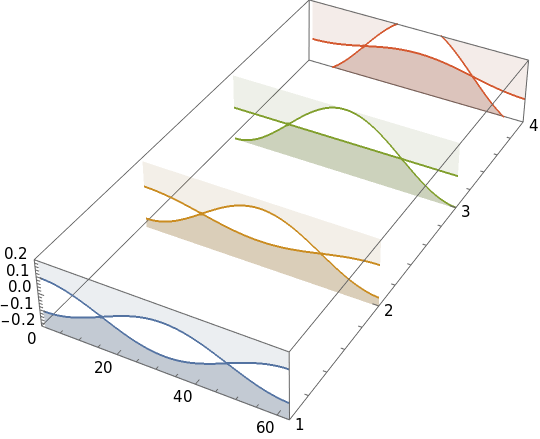
\includegraphics[width=0.7\textwidth]{figures/typeIIridgeline}
  \caption{\label{fig:ridgeline} \todo{Write this} The values of the parameters were chosen to be \(m=0.15, t=-0.05, \) and \(2 k_{0}=\pi\).}
\end{figure}

\begin{figure}[ht]
  \centering
  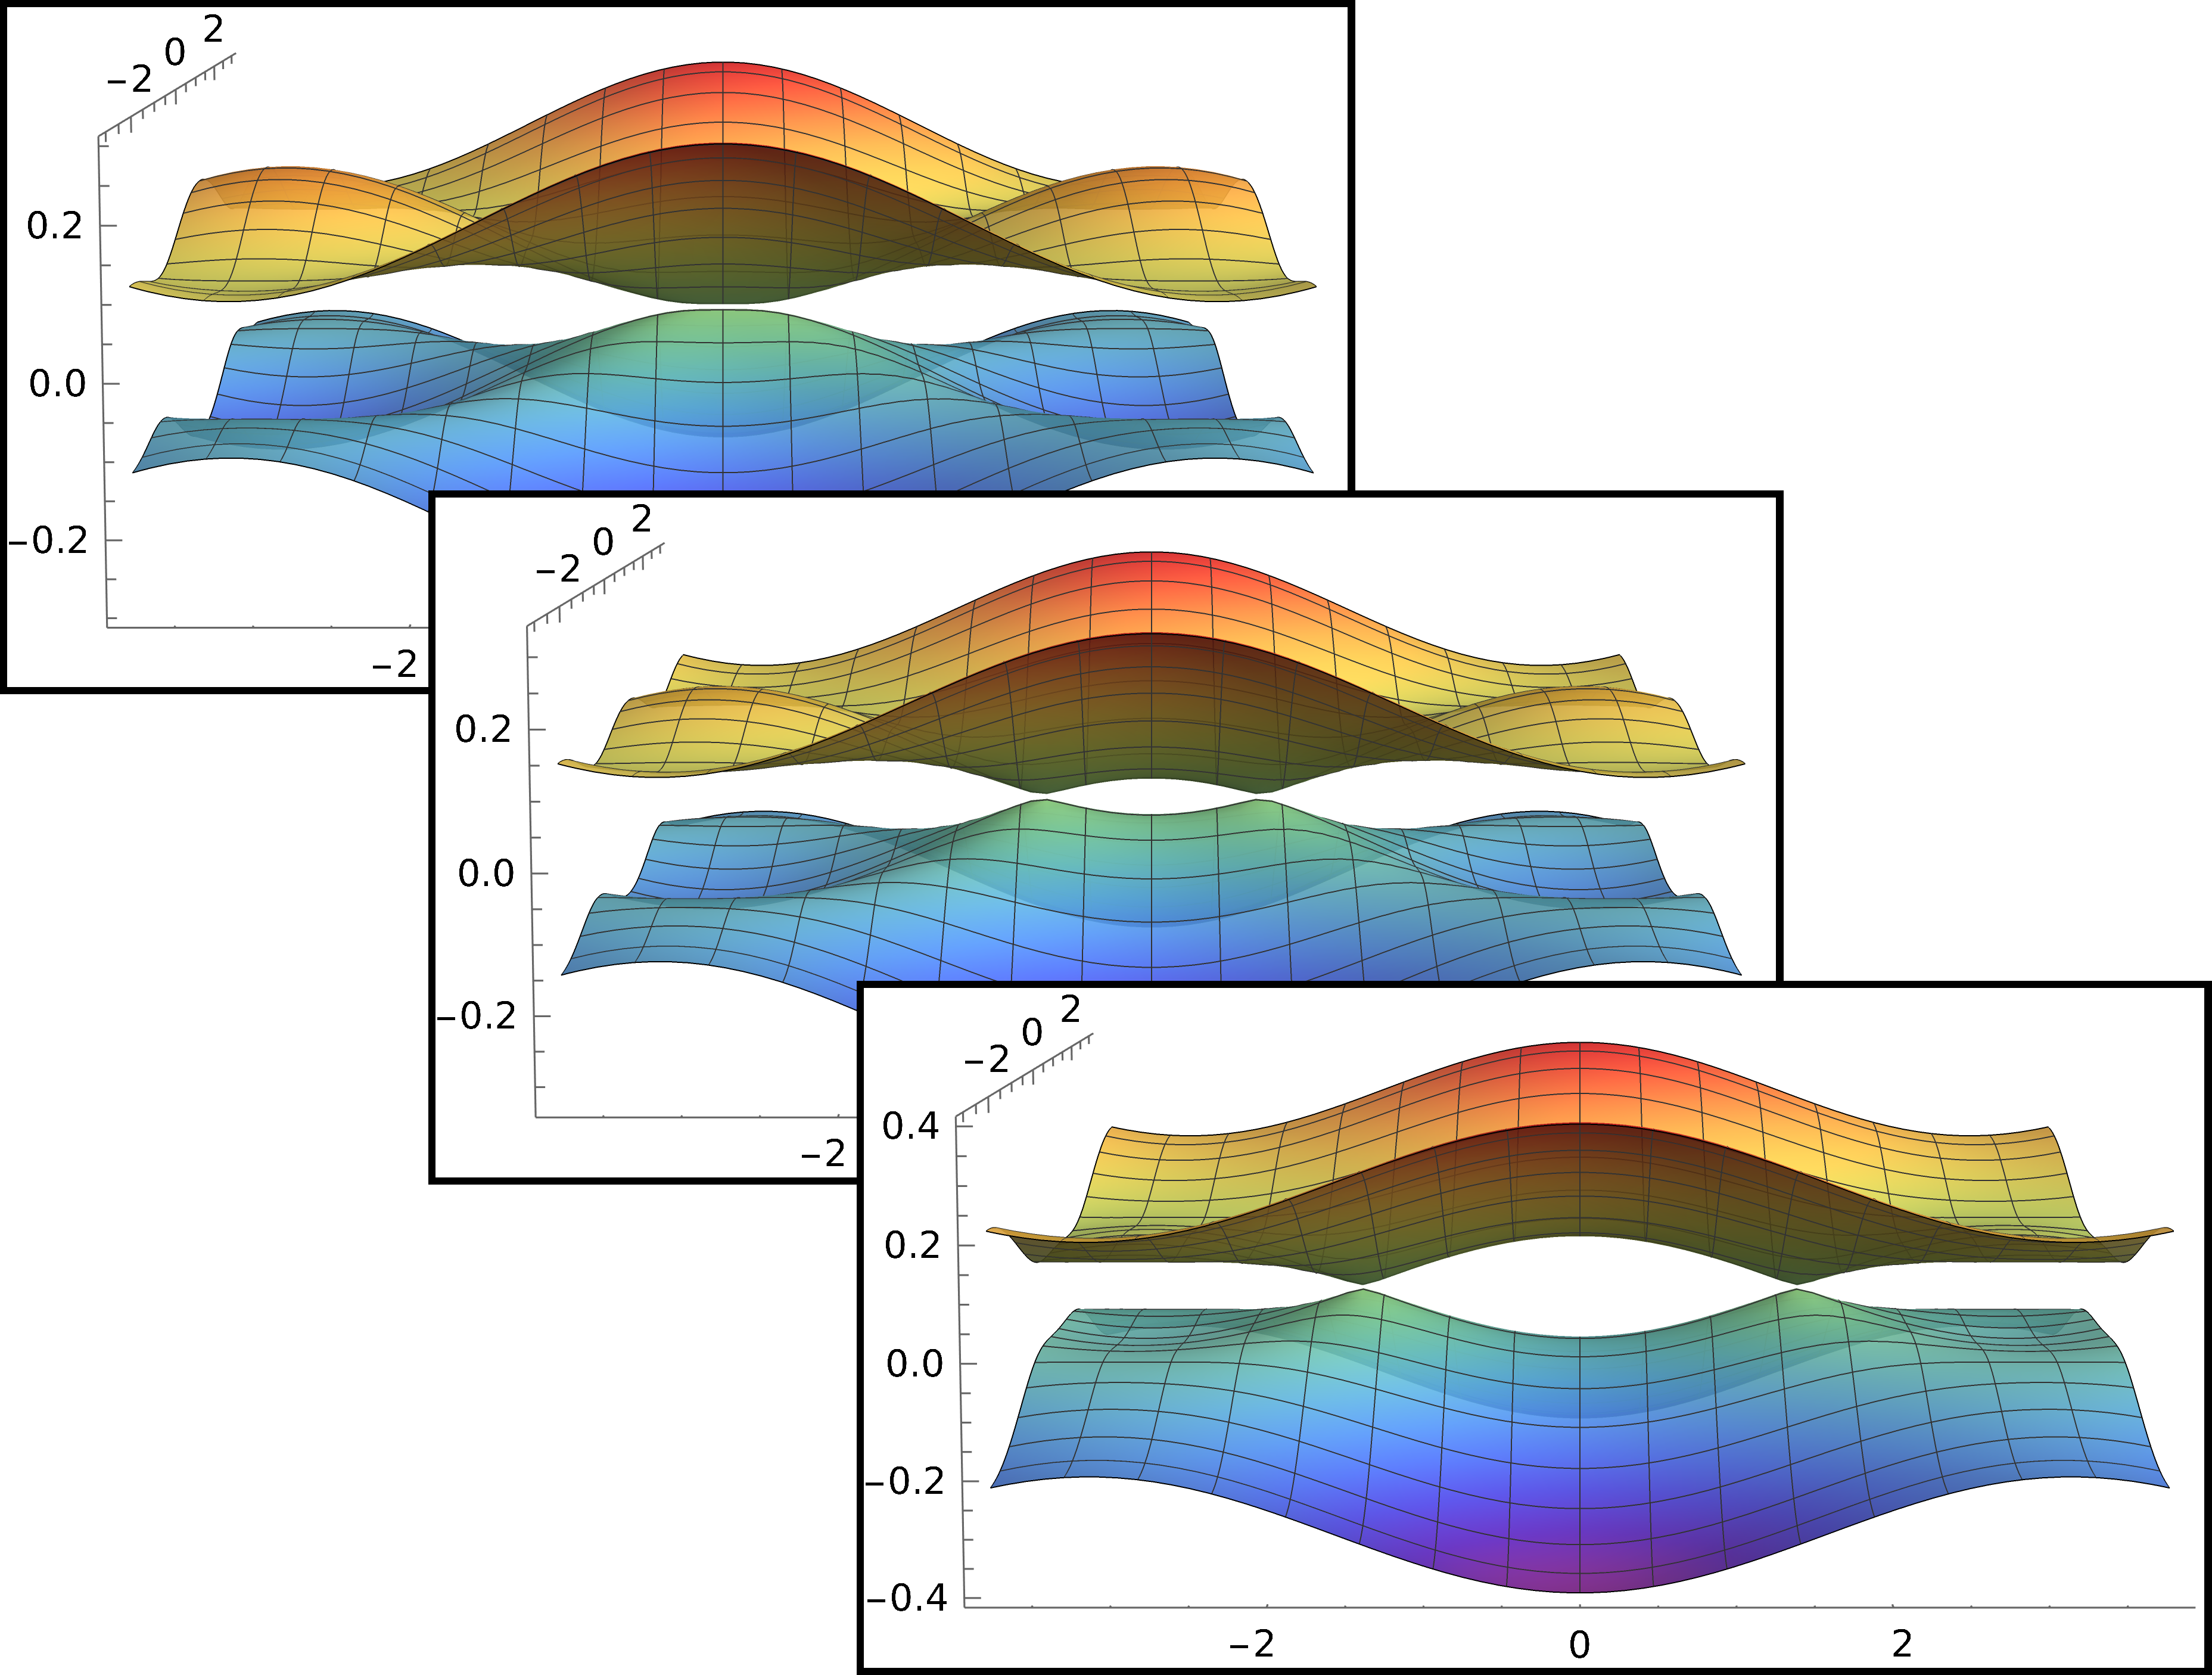
\includegraphics[width=0.7\textwidth]{figures/movetypeiinode}
  \caption{\label{fig:typeii:move-nodes} A Type-II Weyl semimetal with separation between the nodes \(2k_{0} = 0, \pi/2, \pi \).
    See main text for details about the model.}
\end{figure}


\subsection{Eigenstates and Landau levels}
The eigenvalues of Type-II Weyl semimetal simple to find, and are not qualitatively different from those of Type-I, other than the appearence of particle and hole pockets at the Fermi level.
We will also consider the Landau levels of these materials, which importantly are very different from Type-I.
In fact, erroneous treatment of the Landau spectrum of Type-II semimetals caused the original paper describing Type-II materials to mistakenly assert that the chiral anomaly would not be present for certain directions of a background magnetic field \cite{soluyanovTypeIIWeylSemimetals2015}\cite{sharmaChiralAnomalyLongitudinal2017}.

Eigenstates, spin, berry, etc

The issue with the Landau level description is that for certain directions of the \(B\)-field, the levels break down and become imaginary.
For Type-I materials, the description is valid for all dierections of the \(B\)-field, but as the cone tip into a Type-II material, the description breaks down when the \(B\)-field and tilt direction are perpendicular \cite{sharmaChiralAnomalyLongitudinal2017}, and as the magnitude of the tilt is increased, the Landau levels are only valid up to a certain angle between the tilt direction and magnetic field.

Consider the Hamiltonian
\begin{equation}
  \label{eq:4}
  H = \vec{\omega_{0}} \vec{k} + (\vec{v} \odot \vec{k}) \vec{\sigma},
\end{equation}
where \(\vec{\omega_{0}}\) is the tilt vector and \(\vec{v}\) is the Fermi velocity, which in general is anisotropic.
To find the Landau levels in a magnetic field \(\vec{B} = B_{z}\hat{z} \), we will ``Lorentz boost'' the system to a frame where the cone is not tilted, where we may use the usual approach for finding the Landau levels.
Firstly, assume that the tilt vector \(\vec{\omega_{0}}\) is in the \(x,z\)-plane, \(\vec{\omega_{0}} = (\omega_{\perp}, 0, \omega_{\parallel})\), which we can always achieve by a rotation around \(z\).
\todo{Proof by figure}
Introduce the \(\vec{B}\)-field by the minimal coupling \(\vec{k} \to \vec{k}^B = \vec{k} + e \vec{A}\), and use the Landau gague \(\vec{A} = -B_{z}y \hat{x}\).
The Hamitonian can thus be written
\begin{equation}
  \label{eq:5}
  H_{B} = \omega _{\perp} \left(k_{x} - e B_{z} y \right) + \omega _{\parallel} k_{z} + v_{y} k_{y} \sigma _{y} + v_{z} k_{z} \sigma _{z} + v_{x} \left(k_{x} - e B_{z} y\right) \sigma _{x},
\end{equation}
and the Landau level equation is
\begin{equation}
  \label{eq:6}
  \left(H_{B} - E\right) \ket{\psi } = 0.
\end{equation}
In order to use the ladder operator method used for the untilted cone, we must get rid of the \(k^B_{x}\) on the diagonal of the Hamiltonian.
\footnote{It would also be possible to choose the frame such that the tilt was both in \(x\) and \(y\) direction, in which case we would get ladder operators also on the diagonal.
  This system, albeight tedious, could also have been solved directly.
  \todo{Verify this}
}
To achieve this, we will use a ``Lorentz transformation'', which as we will show only leave \(k_{z}\) and \(E\) in the diagonal.
Act with the hyperbolic rotation operator \(\exp[\Theta /2 \sigma_{x}]\) on Eq. \eqref{eq:6}, and insert identity on the form \(\exp[\Theta /2 \sigma_{x}]\exp[-\Theta /2 \sigma_{x}]\) before the state vector.
By introducing the state in the rotated frame \(\ket{\tilde{\psi}} = \exp[- \Theta /2 \sigma_{x}] \mathcal{N} \ket{\psi } \), with \(\mathcal{N}\) a normalization factor compensating for the non-unitarity of the transformation, we get the eigenvalue equation
\begin{equation}
  \label{eq:7}
  (\exp[\Theta /2 \sigma_{x}] H_{B}\exp[\Theta /2 \sigma_{x}] - E \exp[\Theta \sigma_{x}]) \ket{\tilde{\psi}} = 0.
\end{equation}

We rewrite the Hamiltonian (Eq. \eqref{eq:5}) in a more compact and explicit way
\begin{equation}
  \label{eq:8}
  H_{B} = \left(\omega _{\perp} k^B_{x} + \omega _{\parallel} k^B_{z} \right) \mathcal{I}_2 + \sum_i v_{i} k^B_{i} \sigma _{i},
\end{equation}
where \(\mathcal{I}_{2}\) is the identity matrix of size 2.
We now make the fortunate observation that, with the hyperbolic rotation operator denoted \( R = \exp [\Theta / 2 \sigma_{x}]\), the diagonal elements of
\[
R \sigma_{i} R
\]
are zero for $i=y$ and non-zero for \(i=x,z\).
We may thus rotate the \(x\) and \(z\) in and out of the diagonal elements, without accidentaly rotating the \(y\) components into the diagonal.

The problematic part of the Hamiltonian with regards to finding the Landau levels, are the terms containing \(k^B_{x}\) on the diagonal, i.e.
\[
  \omega _{\perp} k^B_{x} \mathcal{I}_{2} + v_{x} k^B_{x} \sigma _{x}.
\]
We will now find the boost parameter that eliminates \(q_{x}\) from the diagonal.
We have
\begin{equation}
  \label{eq:9}
  R^{2} = e^{\Theta \sigma _{x} } =
  \begin{pmatrix}
    \cosh \theta & \sinh \theta \\
    \sinh \theta & \cosh \theta
  \end{pmatrix}
\end{equation}
and as $[R, \sigma_{x}] = 0$,
\begin{equation}
  \label{eq:10}
  R \sigma _{x} R =  R^{2} \sigma _{x} =
  \begin{pmatrix}
    \sinh \theta & \cosh \theta \\
    \cosh \theta & \sinh \theta
  \end{pmatrix},
\end{equation}
as the effect of \(\sigma _{x}\) is to transpose the rows.
The requirement for \(k^B_{x}\) to be rotated out of the diagonal is thus
\begin{equation}
  \label{eq:11}
  \omega _{\perp} \cosh \theta + v_{x} \sinh \theta = 0.
\end{equation}
Solving for \(\theta \) we get
\begin{equation}
  \label{eq:12}
  \theta = \log (
  \pm \frac{\sqrt{v_{x} - \omega _{\perp}}}{\sqrt{v_{x} + \omega _{\perp}}}
  ).
\end{equation}
\todo{NB: depending of choice of sign in log, we get different signs in answer}
Alternatively, written in a slightly suggestive form,
\begin{equation}
  \label{eq:13}
  \tanh \theta =
  - \frac{\omega _{\perp}}{v_{x}}.
\end{equation}
\todo{For pedagogic reasons, include arctanh, which is only valid for -1 < x < 1, explicitly showing the collapse?}

Before we proceed any further, we will put the above into a more solid context, defining some useful quantities and more carefully investigte what is going on, which will be of help later when considering for the regions of validity, and the physical reason behind it.

\todo{nice plot of the landau levels acutally being squeezed}

Introduce the dimensionless \emph{tilt parameter}
\[
  \vec{t} =
  \left(
  \frac{\omega_{0x}}{v_{x}},
  \frac{\omega_{0y}}{v_{y}},
  \frac{\omega_{0z}}{v_{z}}
\right).
\]
Let also \(v_{i} = v_{0} a_{i}\), where \(\vec{a}\) is a vector describing the anisotropy of the system.
In these parameters, the eigenvalues of the system are
\begin{equation}
  \label{eq:14}
  E(\vec{k}) = \vec{\omega_{0}} \vec{k} \pm \sqrt{(v_{i} k_{i})^{2}} = \sqrt{(t_{i} v_{i} k_{i})^{2}} \pm \sqrt{(v_{i} k_{i})^{2}}.
\end{equation}
The system is Type-II if the first term dominates for any \(\vec{k}\), and Type-I if the last term dominates \cite{soluyanovTypeIIWeylSemimetals2015}.
The \(\vec{t}\)-vector is thus a convenient tool for categorization -- if \(t > 1\) we have a Type-II, else we have a Type-I.
\begin{proof}
  We may always rotate our coordinate system such that, without loss of generality, \(\vec{t} = t \hat{x}\).
  In that case, the first term obviously dominates in the \(x\)-direction, when $t>1$.
\end{proof}


Expressed in the parameter \(t\), the result in Eq. \eqref{eq:13} has an intuitive, and quite visual, interpretation.
As described above, we have rotated our frame such that the tilt is confined to the \(x,z\)-plane, i.e. no tilt in the \(y\)-direction.
The required hyperbolic tilt angle to eliminate the \(k^B_{x}\) in the diagonal elements of the Hamiltonian, originating from the tilt, was
\begin{equation}
  \label{eq:15}
  \theta = - \tanh^{-1} \frac{\omega_{\perp}}{v_{x}} = - \tanh^{-1} t_{x}.
\end{equation}
The inverse of \(\tan \), of course, diverges as the argument approaches \(\pm 1\), as shown in Figure \ref{fig:arctanh}.
\begin{figure}[ht]
  \centering
  % \includegraphics[options]{figures/path.pdf}
  \begin{tikzpicture}
    \pgfkeys{/pgf/declare function={arctanh(\x) = 0.5*(ln((1+\x)/(1-\x)));}}
    \begin{axis}[
      xmin=-1.2, xmax=1.2,
      ymin=-3.9, ymax=3.9,
      samples=200,
      enlarge x limits=false,
      grid=both,
      no markers,
      % axis equal
      xlabel=\(x\),
      ylabel=\(\tanh^{-1} x\),
      % ytick=none,
      ]
      \addplot +[thick,domain=-0.999:0.999] {arctanh(x)};
      \draw [thick,dashed,domain=-0.99:0.99] (1,-4) -- (1,4);
      \draw [thick,dashed,domain=-0.99:0.99] (-1,-4) -- (-1,4);
    \end{axis}
  \end{tikzpicture}
  \caption{\label{fig:arctanh} Plot of \(\tanh^{-1}\), which diverges as the argument goes to \(\pm 1\).}
\end{figure}
For \(t_{x} < 1\) we are able to find an angle \(\theta \) which transforms our Hamiltonian into a form which we may solve.
For \(t_{x} \geq 1\), however, no (real) solution of \(\theta \) exits, and the Landau level description collapses.
\todo{ Is this argumentation sufficient? What if we just have to use a different approach to find the LLs? }
It is also interesting that there are no restrictions on the tilt in \(z, t_{z}\).
Visually, this can be visualized by plotting the \(t\)-vector inside a unit sphere.
If the vector is outside the unit sphere, it is a Type-II, if it is inside, it is a Type-I.
Also, if the projection of the vector onto the \(x,y\)-plane is on the unit disk, the Landau level description is valid, if not, the Landau levels collapse.
All Type-I materials may thus be described by Landau levels, while it for Type-II is only valid for certain directions of the \(t\)-vector.
As the \(t\)-vector gets larger, the region of valid directions is reduced to an ever smaller cone around \(z\).
\begin{figure}[ht]
  \centering
  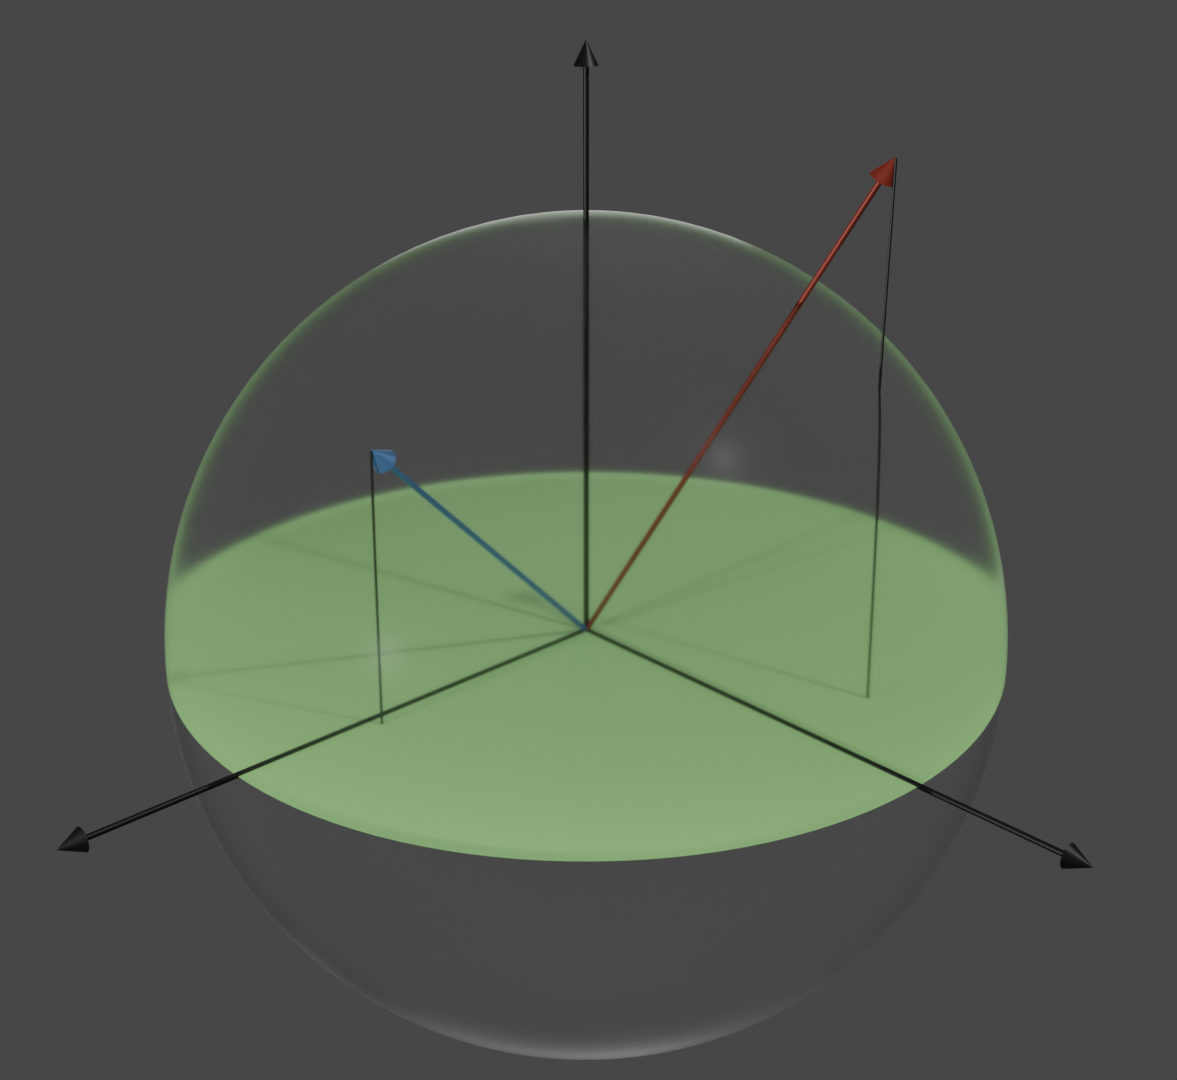
\includegraphics[width=0.75\textwidth]{figures/tiltSpherewBackground.png}
  \caption{\label{fig:tiltSphere} TODO}
\end{figure}

We now return to solving Eq. \eqref{eq:7}, using the solution angle we just found.
By insertion, and after some clean up, we get
\emph{note to thorvald: we chose \(\theta = Log \left(+ \dots\right) \)}
\begin{equation}
  \label{eq:16}
  =
  \begin{pmatrix}
    k_z (v_{z} + \omega_{\parallel} \gamma) - E \gamma   & -i k_{y} v_{y} + \gamma k^{B}_{x} (v_{x} - \frac{\omega_{\perp}^{2}}{v_{x}}) + E \omega_{\perp} \gamma /v_{x} - k_{z} \omega _{\perp} \omega _{\parallel} \gamma /v_{x}\\
    i k_{y} v_{y} + \gamma k^B_{x} (v_{x} - \frac{\omega_{\perp}^{2}}{v_{x}}) + E \omega_{\perp} \gamma /v_{x} - k_{z} \omega _{\perp} \omega _{\parallel} \gamma  / v_{x}
    & -k_{z} (v_{z} - \omega_{\parallel} \gamma) - E \gamma
  \end{pmatrix}.
\end{equation}
after some more clean up
\begin{equation}
  \label{eq:17}
  =
  \begin{pmatrix}
    k_z (v_{z} + \omega_{\parallel} \gamma) - E \gamma   & -i k_{y} v_{y} + v_{x} k^B_{x} / \gamma  - E  \gamma \beta  + k_{z} \omega _{\parallel} \gamma \beta \\
    i k_{y} v_{y} + v_{x} k^B_{x} / \gamma  - E  \gamma \beta  + k_{z} \omega _{\parallel} \gamma \beta
    & -k_{z} (v_{z} - \omega_{\parallel} \gamma) - E \gamma
  \end{pmatrix}.
\end{equation}
In order to simplify this further, absorb \(\gamma \beta \frac{k_{z} \omega_{\parallel} - E}{v_{x}}\) into \(k_{x}\).
Also, we will rescale all momenta to make the effective Fermi velocity isotropic.
Thus, let
\begin{equation}
  \begin{split}
    \tilde{k}_{x} &= \frac{v_{x}}{v_{F}} \left[  k_{x} / \gamma + \gamma \beta \frac{k_{z} \omega_{\parallel} - E}{v_{x}} \right],\\
    \tilde{k}_{y} &= \frac{v_{y}}{v_{F}} k_{y},\\
    \tilde{k}_{z} &= \frac{v_{z}}{v_{F}} k_{z}.\\
  \end{split}
\end{equation}
The eigenvalue equation is simply
\begin{equation}
  \label{eq:18}
  v_{F} \left[  \gamma \left( \frac{\omega_{\parallel}}{v_{z}} \tilde{k}_{z} - \frac{E}{v_{F}} \right) \mathcal{I}_{2} +
  \tilde{k}_{i} \sigma _{i} \right] \ket{\tilde{\psi}}= 0.
\end{equation}
If we now again introduce the magnetic field using minimal coupling, \(k_{x} \to  k_{x} - ey B_{z} \), this corresponds to an effective field \(B_{z} \frac{v_{x} v_{y}}{v_{F}^2} / \gamma \) in the new quantities.
This is because \(\tilde{k}_{x} \to  \tilde{k}_{x} - e \tilde{y} \frac{v_{y} v_{x}}{v_{F}^2}  B_{z} /\gamma \), where the rescaled \(\tilde{y} = \frac{v_{F}}{v_{y}} y\).

The Landau level equation thus reads
\begin{equation}
  \label{eq:19}
  \left[
  \sum\limits_{i} v_{F} \left(\tilde{k}_{i} + e \tilde{A}_{i} \right) \sigma _{i}
\right  ] \ket{\tilde{\psi}} =
(E- t_{\parallel} v_{F} \tilde{k}_{z}) \gamma \ket{\tilde{\psi}},
\end{equation}
where \(\vec{\tilde{A}}=-B_{z} \frac{v_{x} v_{y} }{v_{F}^2} / \gamma  \tilde{y} \hat{x}\).
We may thus use directly the result for the untilted cone, \todo{eq ref}, giving
\begin{align}
  \label{eq:20}
  \left(E - t_{\parallel} v_{F} \tilde{k}_{z} \right) \gamma &= \sign (m) v_{F} \sqrt{2 |m| e \frac{B v_{x} v_{y}}{ v_{F} ^2 \gamma } \hbar + \tilde{k}_{z}^2 \hbar ^2}, & m \neq 0,\\
  \left(E - t_{\parallel} v_{F} \tilde{k}_{z} \right) \gamma &= - s \hbar  \tilde{k}_{z} v_{F}, & m=0.
\end{align}
Cleaning up, we get
\begin{align}
  \label{eq:21}
  E &= t_{\parallel} v_F \tilde{k}_{z} + \sign(m) \sqrt{2 |m| e \frac{v_{y} v_{x} B}{\gamma ^3} \hbar + v_{F}^2 \tilde{k}_{z}^2\hbar ^2 /\gamma ^2}, & m\neq 0,\\
  E &= \tilde{k}_{z} v_{F} \left( t_{\parallel}  - s \hbar / \gamma  \right), & m=0.
\end{align}

As the tilt is increased, \(\gamma = 1 / \sqrt{1-\beta ^{2}}\) diverges to infinity.
With the trivial substitution \(\alpha = \frac{1}{\gamma }\), which goes to zero, this gets an intuitive interpretation.
\begin{equation}
  \label{eq:22}
  E = t_{\parallel} v_{F} \tilde{k}_{z} + \sign(m)  \sqrt{2 |m| e B v_{x} v_{y} \alpha  ^3 \hbar + v_{F} ^2 \tilde{k}_{z}^2\hbar ^2 \alpha ^2}
\end{equation}
As the tilt increases, the Landau levels converge towards \(t_{\parallel} v_{F} \tilde{k}_{z}\).
\todo{Note that \( \tilde{k}\to 0 \) as we overtilt as well, so all the levels go to zero.}
In particular, the separation between Landau levels \(m\) \todo{maybe use the word cyclotron frequency} is reduced by a factor \(\alpha ^{\frac{3}{2}}\).
The effect of the tilt on the Landau levels is to squeeze the Landau levels together, and we will call the \(\alpha ^{\frac{3}{2}}\) the \emph{squeezing factor}.
We note that when approaching the degree of tilt where we are no longer able to find a boost which enables us to solve for the Landau levels, i.e. when \(\beta \to 1\), the squeezing factor goes to zero.
As the tilt exceeds this limit, the squeezing factor is imaginary.

Consider now isotropic velocities \( v_i = v_F \).
Even for anisotripic systems, we may rescale the momenta to arrive at such a description.
We may rewrite the energy as
\[
  E =
  \begin{cases}
    t_{\parallel} v_F k_z + \operatorname{sign}(m) v_F \alpha \sqrt{2 |m| e B \alpha + k_z^2} & m\neq 0\\
    t_{\parallel} v_F k_z - s \alpha v_F k_z & m=0,
  \end{cases}
\]
where \( \hbar = 1 \).
Notice that this is exactly
\[
E = t_{\parallel} v_F k_z + \alpha E^0_{m, \alpha B},
\]
where \( E^0_{m, B} \) is the energy in the untilted case, with magnetic field \( \alpha B \).

The eigenstate of
\[
H = v_{F} \sigma ^{i} ( p_{i} + e A_{i} ),
\]
with \(A_{i} = - B_{z} y \delta _{i x}\), given in the position basis, is
\begin{equation}
  \phi _{\vec{k} m s}(\vec{r}) = \frac{1}{\sqrt{L_xL_z}}
  \frac{e^{ik_x x}e^{ik_z z}}{\sqrt{\alpha _{k_z m s}^2 + 1}}
  e^{-\frac{y-k_x l^2}{2 l_B^2}}
  \begin{pmatrix}
    \frac{\alpha _{k_z m s}}{\sqrt{2^{M-1} (M-1)! \sqrt{\pi } l_B}} H_{M-1}\left( \frac{y-k_x l_B^2}{l_B} \right)\\
    \frac{1}{\sqrt{2^M M! \sqrt{\pi } l_B}} H_M \left( \frac{y-k_x l_B^2}{l_B} \right)
  \end{pmatrix},
\end{equation}
where capital letters indicate absolute value of corresponding quantity, $M=|m|, \vec{k} = (k_x, k_z)$, and with the normalization factor
\begin{equation}
  \alpha _{k_z m s} = \frac{-\sqrt{2eB\hbar M}}{\frac{E_{k_z m s}}{s v_{F}} - \hbar  k_z}.
\end{equation}
Taking care to keep track of boosted and rescaled quantites, the eigenstate in the boosted frame is
\begin{equation}
  \label{eq:29}
  \tilde{\psi}(\tilde{\vec{r}}) =
  \frac{1}{\sqrt{L_xL_z}}
  \frac{e^{i \tilde{k}_x \tilde{x}}e^{i k_z z}}{\sqrt{\alpha _{\tilde{k}_z m s}^2 + 1}}
  e^{-\frac{\left(\tilde{y} - \tilde{k}_x l_{B'}^2\right)^2}{2 l_{B'}^2}}
  \begin{pmatrix}
    \frac{\alpha _{\tilde{k}_z m s}}{\sqrt{2^{M-1} (M-1)! \sqrt{\pi } l_{B'}}} H_{M-1}\left( \frac{\tilde{y} - \tilde{k}_x l_{B'}^2}{l_{B'}} \right)\\
    \frac{1}{\sqrt{2^M M! \sqrt{\pi } l_{B'}}} H_M \left( \frac{\tilde{y} - \tilde{k}_x l_{B'}^2}{l_{B'}} \right)
  \end{pmatrix},
\end{equation}
with
\begin{equation}
  \alpha _{\tilde{k}_z m s} = \frac{-\sqrt{2e B' \hbar M}}{ \gamma \frac{E_{\tilde{k}_z m s} - t_{\parallel} v_{F} \tilde{k}_{z}}{s v_{F}} - \hbar  \tilde{k}_z},
\end{equation}
where \(E\) is the solution in the unboosted frame and
\[
B' = B \frac{v_{x} v_{y}}{v_{F}^2} \alpha
\]


And thus the original eigenstate \(\ket{\psi } = 1 /\mathcal{N} e^{\theta /2 \sigma _{x}} \ket{\tilde{\psi} }\) of the tilted system is easily found.

\todo{ Write down the full form of \( \phi _{\vec{k} m s} (\vec{r}) \), taking care to use the original momenta, and not the rescaled. }

Reinserting explicitly, in the boosted frame, that \(\tilde{q}_{x} = \alpha q_{x} + \frac{\beta}{\alpha } \frac{k_{z} \omega _{\parallel} - E}{v_{x}} \) and \(l_{B'}=\frac{l_{B}}{\sqrt{\alpha} }\)
\todo{note we have used isotropic velocity}
we get
\begin{equation}
  \label{eq:41}
  \frac{y-\tilde{q}_{x} l_{B'}^2}{l_{B'}}
  =
  \frac{y - \alpha q_{x} l_{B'}^2 - \frac{\beta l_{B'}^2}{\alpha } \frac{k_{z} \omega _{\parallel} - E}{v_{x}}}{l_{B'}}
  =
  \sqrt{\alpha } (y-q_{x} l_{B}^2) /l_{B} - \alpha^{-\frac{3}{2}}  \beta l_{B} \frac{k_{z} \omega _{\parallel} - E}{v_{x}}.
\end{equation}
Using the explicit form of \(E\)
\begin{equation}
  \label{eq:43}
  \chi =
  \frac{y-\tilde{q}_{x} l_{B'}^2}{l_{B'}}
  =
  \sqrt{\alpha } (y-q_{x} l_{B}^2) /l_{B}
  + \frac{ \beta l_B }{ \sqrt{\alpha}} E^{0}_{m, \alpha B},
\end{equation}.
\todo{ Clean up in \(\hbar \) }


\begin{equation}
  \label{eq:40}
  \tilde{\phi} _{\vec{k} m s} (\vec{\tilde{r}})
  =
  \frac{1}{\sqrt{L_xL_z}}
  \frac{e^{i \tilde{k}_x \tilde{x}}e^{i k_z z}}{\sqrt{\alpha _{\tilde{k}_z m s}^2 + 1}}
  e^{-\frac{1}{2} \chi ^2}
  \sqrt[4]{\alpha }
  \begin{pmatrix}
    \frac{\alpha _{\tilde{k}_z m s}}{\sqrt{2^{M-1} (M-1)! \sqrt{\pi } l_{B}}} H_{M-1}\left( \chi  \right)\\
    \frac{1}{\sqrt{2^M M! \sqrt{\pi } l_{B}}} H_M \left( \chi \right)
  \end{pmatrix}.
\end{equation}
For later convenience, let us explicitly define
\begin{equation}
  \label{eq:32}
  \tilde{\phi} _{\vec{k} m s} (\vec{\tilde{r}}) =
  \frac{e^{i \tilde{k}_{x} \tilde{x} + i k_{z} z}}{\sqrt{L_{x} L_{z}} }
  \underbrace{
  \frac{
    e^{-\frac{1}{2} \chi ^2}
    \sqrt[4]{\alpha }
  }
  {\sqrt{\alpha^2_{\tilde{k}_{z} m s} + 1} }
  \begin{pmatrix}
    \frac{\alpha _{\tilde{k}_z m s}}{\sqrt{2^{M-1} (M-1)! \sqrt{\pi } l_{B}}} H_{M-1}\left( \chi  \right)\\
    \frac{1}{\sqrt{2^M M! \sqrt{\pi } l_{B}}} H_M \left( \chi \right)
  \end{pmatrix}}_{\tilde{\phi}_{\vec{k} m s} (y)},
\end{equation}
and thus
\begin{equation}
  \label{eq:42}
  \tilde{\phi}_{\vec{k} m s} (y) =
  e^{-\frac{1}{2} \chi ^2}
  \begin{pmatrix}
    a_{\vec{k} m s} H_{M-1} (\chi)\\
    b_{\vec{k} m s} H_{M} (\chi)
  \end{pmatrix},
\end{equation}
with
\begin{align}
  a_{\vec{k} m s} &=
                    \frac{
                    \alpha _{\tilde{k}_z m s} \sqrt[4]{\alpha }
                    }{
                    \sqrt{\alpha^2 _{\tilde{k}_z m s} + 1}
                    \sqrt{2^{M-1} (M-1)! \sqrt{\pi} l_B}
                    },\\
  b_{\vec{k} m s} &=
                    \frac{
                     \sqrt[4]{\alpha }
                    }{
                    \sqrt{\alpha^2 _{\tilde{k}_z m s} + 1}
                    \sqrt{2^{M} M! \sqrt{\pi} l_B}
                    }.\\
\end{align}


Repeating the calculation of the response function is now straightforward, but rather tedious.
Due to the boost transformation, the elements of the spinor in the untilted system, Eq. \eqref{eq:29}, mix.
We thus have twice as many terms to keep track of.

Consider the expression for the current operator, Eq. 4.39, which we derived form the time evolution relation
\[
  \dot{A} = [A, H]/i\hbar,
\]
by considering \(\vec{v} = \vec\dot{r}\), as \(\vec{J} = e \vec{v}\).
In the tilted Hamiltonian, the tilt term thus causes another term in the current operator.
\begin{equation}
  \label{eq:36}
  \begin{split}
    \vec{v} = \vec\dot{r} &= \frac{1}{i \hbar } [\vec{r}, H] \\
    &= \frac{s v_{F} \sigma ^{ i}}{i \hbar } [\vec{r}, p_{i} + e A_{i}] + \frac{1}{i\hbar } [\vec{r}, \omega_{0} \vec{k}]\\
    &= \frac{s v_{F} \sigma ^{ i}}{i \hbar } (i\hbar + e[\vec{r}, A_{i}]) + \vec{\omega}_{0}\\
    &= s v_{F} \sigma ^{i} + \vec{\omega} _{0}.
  \end{split}
\end{equation}

Take for example the matrix element of the current operator
\[
  J_{\vec{k} m s; \vec{k}+\qvec{q} n s } (\vec{q}) = \int \mathrm{d}y e^{-i q_{y} y}
  s v_{F} e \phi ^{*}_{\vec{k} m s} (y) \sigma ^{x} \phi _{\vec{k} + \qvec{q} n s}(y).
\]
We must find the matrix product \(\phi \sigma_{x} \phi \).
Recall that \(\phi = \frac{1}{\mathcal{N}} e^{\theta /2 \sigma _{x}} \tilde{\phi} \), and thus we must find
\[
  \phi ^{*} \sigma _{x} \phi = \frac{1}{\mathcal{N}^{*} \mathcal{N}} \tilde{\phi}^{*} e^{\theta /2 \sigma _{x}} \sigma _{x} e^{\theta /2 \sigma _{x}} \tilde{\phi} =  \frac{1}{\mathcal{N}^{*} \mathcal{N}} \tilde{\phi}^{*} \sigma _{x} e^{\theta \sigma _{x}} \tilde{\phi}.
\]
With the previously found solution \(\theta = - \tanh ^{-1} t_{x}\), we get the rather simple form
\[
  e^{\theta \sigma _{x}} =
  \begin{pmatrix}
    1 & -t_{x}\\
    -t_{x} & 1
  \end{pmatrix}
  \frac{1}{\sqrt{1-t_{x}^2}}.
\]
With
\begin{equation}\label{eq:45}
  \tilde{\phi} = e^{-\frac{1}{2} \chi ^2}
  \begin{pmatrix}
    a_{\vec{k} m s} H_{M-1} (\chi)\\
    b_{\vec{k} m s} H_{M} (\chi)
  \end{pmatrix}
\end{equation}
we see how the expressions change when \(t_{x}\) become non-zero.
Where we previoulsy had
\begin{equation}
  \label{eq:27}
  \phi ^{*}_{\vec{k} m s} \sigma _{x} \phi _{\vec{k} + \qvec{q} n s}
  =
  a_{\vec{k} m s} H_{M-1}(\dots) \left[ b_{\vec{k}+\qvec{q} n s} H_{N}(\dots) \right]
  + \dots
\end{equation}
the contents of the square brackets must now include also the other element of the spinor:
\begin{equation}
  \label{eq:28}
  \phi ^{*}_{\vec{k} m s} \sigma _{x} e^{\theta \sigma _{x}} \phi _{\vec{k} + \qvec{q} n s}
  =
  a_{\vec{k} m s} H_{M-1}(\dots)
  \left[
    b_{\vec{k}+\qvec{q} n s} H_{N}(\dots)
    - t_{x} a_{\vec{k} + \qvec{q} n s} H_{N-1} (\dots)
  \right]
  \frac{1}{\sqrt{1-t_{x}^2}}
  + \dots .
\end{equation}

First of all, let us consider the exponent of the product.
Due to the extra term in \(\chi\), this becomes more elaborate.
The exponent is of course
\begin{equation}
  \label{eq:46}
  \exp\{-i q_{y} y - \frac{1}{2} \chi_{\vec{k}} ^2 - \frac{1}{2} \chi _{\vec{k} + \qvec{q}}^2\}
\end{equation}
A straightforward but tedious calculation shows that the argument of the exponent can be written as
\begin{equation}
  \label{eq:47}
  -\frac{\alpha}{l_{B}^2} \left(y + \frac{l_{B}^2}{2 \alpha } (i q_{y} - (q'_x + 2 k'_x))\right)^2
  -\frac{l_{B}^2}{4 \alpha } (q_{y}^2 + 2i (q'_x + 2 k'_x) q_{y} + ( q' _{x} )^2 ),
\end{equation}
where we have defined
\begin{align}
  q' _x &= \frac{q_x}{\alpha } + \frac{\beta}{v_{F} \alpha }( E^0_{n,\alpha B} - E^0_{m, \alpha B} ),\\
  k' _x &= \frac{k_x}{\alpha } + \frac{\beta}{v_F \alpha } E^0_{m, \alpha B}.
\end{align}
\begin{align}
  A &= k_{x} + \frac{\beta}{l_{B} \sqrt{\alpha }} \sign(m) \sqrt{\frac{k_{z}^2l_{B}^2}{\alpha } + 2 M}\\
  B &= k_{x} + q_{x} + \frac{\beta}{l_{B} \sqrt{\alpha }} \sign(n) \sqrt{\frac{k_{z}^2l_{B}^2}{\alpha } + 2 N}
\end{align}
Eq. \eqref{eq:47} is on the same for as in the untilted cone case, and we may thus proceed with the same method.
Make a change of variable
\[
\tilde{y} = \frac{\sqrt{\alpha }}{l_{B}} \left(y + \frac{l_{B}^2}{2\alpha } (iq_{y} - 2 k' _x - q' _x )\right),
\]
\todo{Follow up the substitiuoin of the root in the integral. Consider moving the root into \(\Xi \)}
to get the exponent on the form \(e^{-\tilde{y}^2}\).
With this substitution,
\begin{align}
  \chi _{\vec{k}} &= \tilde{y} + \frac{l_{B}}{2 \sqrt{\alpha }} \left(q' _x - i q_{y}\right)\\
  \chi _{\vec{k} + \qvec{q}} &= \tilde{y} + \frac{l_{B}}{2 \sqrt{\alpha }} \left(- q' _x - i q_{y}\right)
\end{align}

Doing this, Eq. (4.59) \todo{fix ref} in the project thesis, becomes
\begin{equation}
  \label{eq:28}
  \begin{split}
    J_{\vec{k}ms; \vec{k}+\qvec{q} ns}(\vec{q}) &=
    \frac{s v_F e}{\sqrt{\alpha }} \int \mathrm{d}\tilde{y} \: l_B
    \exp \left[
      -\frac{l_{B}^2}{4 \alpha } \left(q_{y}^2 + 2i (2 k' _x + q' _x) q_{y} + k'_x^2 \right)
    \right]
    (1-t_{x}^2)^{-\frac{1}{2}}\\
    e^{-\tilde{y}^2}
   &\left[
    a_{\vec{k}ms}b_{\vec{k} + \qvec{q} ns}
    H_{M-1} \left(  \chi_{\vec{k}} \right)
    H_N\left( \chi_{\vec{k} + \qvec{q}} \right) \right.\\
    &- t_{x} a_{\vec{k}ms}a_{\vec{k} + \qvec{q} ns}
    H_{M-1} \left( \chi_{\vec{k}} \right)
    H_{N-1}\left( \chi_{\vec{k} + \qvec{q}} \right)\\
   & +
    b_{\vec{k}ms} a_{\vec{k} + \qvec{q} ns}
    H_M \left( \chi_{\vec{k}} \right)
    H_{N-1} \left( \chi_{\vec{k} + \qvec{q}} \right)\\
    &\left. - t_{x}
    b_{\vec{k}ms} b_{\vec{k} + \qvec{q} ns}
    H_M \left( \chi_{\vec{k}} \right)
    H_{N} \left(  \chi_{\vec{k} + \qvec{q}}\right)
    \right].
  \end{split}
\end{equation}

\begin{multline}
  J_{\vec{k} m s; \vec{k} + \qvec{q} n s} (\vec{q}) =
  \frac{s v_{F} e}{\sqrt{\alpha }}
  \frac{
    \exp \left[
      -\frac{l_{B}^2}{4 \alpha } (q_{y}^2 + 2i (2 k'_x + q'_x) q_{y} + k'_x^2 )
    \right]
  }{
    \sqrt{\alpha _{\vec{k} m s}^2 + 1} \sqrt{ \alpha _{\vec{k} + \qvec{q} n s}^2 + 1 }
  } (1-t_{x}^2)^{-\frac{1}{2}}\\
  % \sum\limits_{i=1}^{4} \chi_{i} (\vec{q}, m, n, s)
  \Big[
    \Xi_{1} (\vec{q}, m, n, s)
    + \Xi _{2} (\vec{q}, m, n, s)\\
    - t_x \frac{a_{\vec{k} + \qvec{q} }}{b_{\vec{k} + \qvec{q} n \mp 1}} \Xi _1(\vec{q}, m, n\mp 1, s)
    - t_x \frac{b_{\vec{k} + \qvec{q} }}{a_{\vec{k} + \qvec{q} n \pm 1}} \Xi _2(\vec{q}, m, n\pm 1, s)
  \Big].
\end{multline}

We here used definitions of \( \Xi \) similar to that in the project thesis, but modified to the tilted case.
\begin{equation}
  \label{eq:30}
  \frac{\Xi_1 ( \vec{q}, m, n, s )}{
    \sqrt{\alpha _{\vec{k} m s}^2 + 1}
    \sqrt{\alpha _{\vec{k} + \qvec{q} n s} ^2 + 1}
  }
  =
  \int \mathrm{d} \tilde{y}
  ~e^{-\tilde{y}^2}
  l_{B}
  a_{\vec{k} m s} b_{\vec{k} + \qvec{q} ns}
  H_{M-1} (\chi_{\vec{k}})
  H_N ( \chi _{\vec{k} + \qvec{q}} )
\end{equation}
\begin{equation}
  \label{eq:31}
  \frac{\Xi_2 ( \vec{q}, m, n, s )}{
    \sqrt{\alpha _{\vec{k} m s}^2 + 1}
    \sqrt{\alpha _{\vec{k} + \qvec{q} n s} ^2 + 1}
  }
  =
  \int \mathrm{d} \tilde{y}
  ~e^{-\tilde{y}^2}
  l_{B}
  b_{\vec{k} m s} a_{\vec{k} + \qvec{q} ns}
  H_{M} (\chi_{\vec{k}})
  H_{N-1} ( \chi _{\vec{k} + \qvec{q}} )
\end{equation}
Using that
\begin{equation}
  \label{eq:31}
  a_{\vec{k} m s} b_{\vec{k} +\qvec{q} ns}
  =
  \frac{a_{\vec{k} m s}}{\sqrt{\alpha _{\vec{k} m s} ^2 + 1} \sqrt{\alpha _{\vec{k} + \qvec{q} ns} ^2  + 1}  }
  \left[
  2^{N+M-1} (M-1)! N! \pi l_{B}^2
\right  ]^{-\frac{1}{2}}
\end{equation}


Now we will consider the second term of the current operator.
\begin{equation}
  \label{eq:37}
  J_{\vec{k} m s; \vec{k} + \qvec{q} n s}^{(2)} (\vec{q}) =
  \int \mathrm{d} y
  e^{-iq_{y} y} e
  \phi ^{*}_{\vec{k} m s}(y) \omega _{0 x} \phi _{\vec{k} + \qvec{q} n s}(y).
\end{equation}
Thus
\begin{multline}
  \label{eq:38}
  J_{\vec{k} m s; \vec{k} + \qvec{q} n s}^{(2)} (\vec{q}) =
  \frac{e \omega _{0 x}}{\mathcal{N}^{*} \mathcal{N}}
  \int \mathrm{d} y
  \exp\{-i q_{y} y - \frac{1}{2} \chi_{\vec{k}} ^2 - \frac{1}{2} \chi _{\vec{k} + \qvec{q}}^2\} \\
  \tilde{\phi} ^{*}_{\vec{k} m s}(y) e^{\theta \sigma _{x}} \tilde{\phi} _{\vec{k} + \qvec{q} n s}(y).
\end{multline}
We have
\begin{multline}
  \label{eq:39}
  J_{\vec{k} m s; \vec{k} + \qvec{q} n s}^{(2)} (\vec{q}) =
  \frac{e \omega _{0 x} l_{B}}{\mathcal{N}^{*} \mathcal{N} \sqrt{\alpha}}
  \int \mathrm{d} \tilde{y}
    \exp \left[
      -\frac{l_{B}^2}{4 \alpha } (q_{y}^2 + 2i (2 k'_x + q' _x) q_{y}  + q'_x^2 )
    \right]\\
  e^{-\tilde{y}^2} \big[
    a_{\vec{k} m s} H_{M-1}( \chi _{\vec{k}} ) \left(a_{\vec{k} + \qvec{q} n s} H_{N-1}( \chi _{\vec{k} + \qvec{q}} ) - t_{x} b_{\vec{k} + \qvec{q} n s} H_{N}( \chi _{\vec{k} + \qvec{q}} ) \right)\\
   +
    b_{\vec{k} m s} H_{M}( \chi _{\vec{k}} ) \left(-t_{x} a_{\vec{k} + \qvec{q} n s} H_{N-1}( \chi _{\vec{k} + \qvec{q}} ) + b_{\vec{k} + \qvec{q} n s} H_{N}( \chi _{\vec{k} + \qvec{q}} ) \right)
    \big]
    (1 - t_{x}^2)^{-\frac{1}{2}}.
\end{multline}
Thus,
\begin{multline}
  J_{\vec{k} m s; \vec{k} + \qvec{q} n s}^{(2)} (\vec{q}) =
  \frac{e \omega _{0 x} l_{B}}{\mathcal{N}^{*} \mathcal{N} \sqrt{\alpha } }
  \frac{
    \exp \left[
      -\frac{l_{B}^2}{4 \alpha } (q_{y}^2 + 2i (2 k' _x + q' _x) q_{y} + q'_x^2 )
    \right]
  }{
    \sqrt{\alpha_{\vec{k} m s}^2 + 1} \sqrt{\alpha _{\vec{k}+\qvec{q} n s}^2 + 1}
  }
  (1-t_{x})^{-\frac{1}{2}}\\
  \left[
    \Xi _{3} - t_{x} \Xi _{1}
    - t_{x} \Xi _{2} + \Xi_{4}
  \right].
\end{multline}


\subsubsection{Stress-energy tensor}
Consider now
\begin{equation}
  \label{eq:33}
  T_{\vec{k} + \qvec{q} n s, \vec{k} m s}^{0y(1)} (\vec{q}) =
  \frac{1}{4}
  \int \mathrm{d} y
  e^{i q_{y} y}
  \phi ^{*}_{\vec{k} + \qvec{q} n s}(y) s \sigma ^{y}
  (E_{k \mu  s} + E_{\lambda \nu s} - 2 \mu)
  \phi _{\vec{k} m s} (y).
\end{equation}
As
\begin{equation}
  \label{eq:34}
  % e^{\theta /2 \sigma _{x}} \sigma _{y} e^{\theta /2 \sigma _{x}} = 1
  \sigma _{y} e^{\theta /2 \sigma _{x}} = e^{-\theta /2 \sigma _{x}} \sigma _{y}
\end{equation}
we get the very fortunate result
\begin{equation}
  \label{eq:35}
  \phi^{*} \sigma _{y} \phi = \tilde{\phi}^{*} \sigma _{y} \tilde{\phi}.
\end{equation}
The first term of the stress-energy tensor thus has the exact same form as the untilted case.
Recalling the expression for \(\tilde{\phi}\) from Eq. \eqref{eq:45},
\[
  \tilde{\phi} = e^{-\frac{1}{2} \chi ^2}
  \begin{pmatrix}
    a_{\vec{k} m s} H_{M-1} (\chi)\\
    b_{\vec{k} m s} H_{M} (\chi)
  \end{pmatrix},
\]
where
\[
\chi = \sqrt{\alpha} (y - q_{x} l_{B}^2 ) /l_{B} - \sign(m) \beta \sqrt{2 |m| + \frac{k_{z}^2 l_{B}^2}{\alpha }}.
\]
We thus get
\begin{multline}
  \label{eq:48}
  T_{\vec{k}+\qvec{q} ns, \vec{k} m s}^{0y (1)} (\vec{q}) =
  \frac{is}{4} (E_{k\mu  s} + E_{\lambda \nu s} - 2 \mu)
  \int \mathrm{d} y
  e^{i q_{y} y}
  e^{-\frac{1}{2} (\chi_{\vec{k}+\qvec{q}}^2 + \chi_{\vec{k}} ^2) }\\
  [
  -a_{\vec{k} + \qvec{q} ns} b_{\vec{k} m s} H_{N-1} (\chi_{\vec{k} + \qvec{q}}) H_{M} (\chi_{\vec{k}})
  + b_{\vec{k} + \qvec{q} n s} a_{\vec{k} ms} H_{N}(\chi_{\vec{k} + \qvec{q}}) H_{M-1} (\chi_{\vec{k}})
  ].
\end{multline}
We will perform once again the completion of the square and substituion of \(y\).
The exponent is the same as that which we found for the current operator case, Eq. \eqref{eq:47}, with the change \(q_{y} \to - q_{y}\).
We thus make the change of variables
\begin{equation}
  \label{eq:49}
  \tilde{y} = \frac{\sqrt{\alpha}}{l_{B}} \left(y  - \frac{l_{B}^2}{2 \alpha } (i q_{y} + (2k' _x + q' _x) )\right),
\end{equation}
giving
\begin{align}
  \chi _{\vec{k}} &= \tilde{y} + \frac{l_{B}}{2 \sqrt{\alpha }} \left( q'_x + i q_{y}\right),\\
  \chi _{\vec{k} + \qvec{q}} &= \tilde{y} + \frac{l_{B}}{2 \sqrt{\alpha }} \left( -q' _{x} + i q_{y}\right).
\end{align}
Thus, analogous to Eq. (4.79), we get
\begin{multline}
  \label{eq:50}
  T_{\vec{k} + \qvec{q} n s, \vec{k} m s}^{0y (1)} (\vec{q}) =\\
  \frac{is}{4 \sqrt{\alpha} }
  (E_{k\mu s} + E_{\lambda  \nu  s} - 2 \mu)
  \exp \left[
    -\frac{l_{B}^2}{4 \alpha } (q_{y}^2 + 2i (2 k' _x + q' _x) q_{y} + q' _x^2 )
  \right  ]
  \int \mathrm{d} \tilde{y} l_{B} e^{-\tilde{y}^2}\\
 \Big[
  - a_{\vec{k} + \qvec{q} ns} b_{\vec{k} m s}
  H_{N-1} ( \chi _{\vec{k}} )
  H_{M} ( \chi _{\vec{k} + \qvec{q}} )
  + b_{\vec{k} + \qvec{q} ns } a_{\vec{k} m s}
  H_{N}( \chi _{\vec{k}} )
  H_{M-1} ( \chi _{\vec{k} + \qvec{q}} )
  \Big]
\end{multline}
And thus we have
\begin{align}
  T_{\vec{k} + \qvec{q} n s, \vec{k} m s}^{0y (1)} (\vec{q}) &=
  \frac{is}{4 \sqrt{\alpha} }
  \frac{E_{k\mu s} + E_{\lambda  \nu  s} - 2 \mu}{
    \sqrt{\alpha _{\vec{k} m s}^2 + 1}
    \sqrt{\alpha _{\vec{k} + \qvec{q} n s}^2 + 1}
  }\\
  &\pe \exp \left[
    -\frac{l_{B}^2}{4 \alpha } (q_{y}^2 + 2i ( 2k' _x + q' _x ) q_{y} + q' _x^2)
  \right  ]\\
  &\pe (-\Xi_{2} (\bar{\vec{q}}, m, n, s) + \Xi_{1}(\bar{\vec{q}}, m, n, s)),
\end{align}
where \(\bar{\vec{q}} = (q_{x}, -q_{y}, q_{z})\).

We must now consider the latter parts of the stress energy tensor
\begin{align}
  T_{\vec{k} + \qvec{q} ns, \vec{k} ms}^{0y (2)} (\vec{q}) &=
                                                             + \frac{1}{4} \int \mathrm{d} y
                                                             e^{iq_{y} y} v_{F}
                                                             \phi ^{*}_{\vec{k}+\qvec{q} ns} (y) p_{y} \phi _{\vec{k} m s} (y),\\
  T_{\vec{k} + \qvec{q} ns, \vec{k} ms}^{0y (3)} (\vec{q}) &=
                                                             - \frac{1}{4} \int \mathrm{d} y
                                                             e^{iq_{y} y} v_{F}
                                                             (p_{y} \phi ^{*}_{\vec{k}+\qvec{q} ns} (y))  \phi _{\vec{k} m s} (y).
\end{align}
Firstly, we note that
\[
  [p_{y} , e^{\theta /2 \sigma _{x}}] = 0.
\]
Furthermore, exactly as for the untilted case, the momentum operator acting on the exponential prefactor of \(\phi \) gives contributions proportional to \(q_{x}\).
In the local limit \(q\to  0\) this term vanishes, and we need only consider the effect of the momentum operator acting on the Hermite polynomials.

Denote by \(\tilde{p}_{y}\) the momentum operator \(p_{y}\) acting only on the Hermite polynomial part of \(\phi \).
Furthermore, we will use the property of Hermite polynomials \(\partial _{x} H_{n} (x) = 2 n H_{n-1} (x)\) \cite[Eq.~18.9.25]{NIST:DLMF}.
\begin{align}
  \tilde{p}_{y} \phi _{\vec{k} ms} &=
  -i \hbar
  e^{\theta /2 \sigma _{x}}
  e^{-\frac{1}{2} \chi ^2}
  \partial _{y}
  \begin{pmatrix}
    a_{\vec{k} m s} H_{M-1} (\chi) \\
    b_{\vec{k} ms} H_{M} (\chi)
  \end{pmatrix}\\
                                   &=
                                     -i \hbar
                                     e^{\theta /2 \sigma _{x}}
                                     e^{-\frac{1}{2} \chi ^2}
                                     2 \frac{\partial \chi }{\partial y}
                                     \begin{pmatrix}
                                       a_{\vec{k} m s} (M-1) H_{M-2} (\chi) \\
                                       b_{\vec{k} ms} (M) H_{M-1} (\chi)
                                     \end{pmatrix}\\
                                   &=
                                     -i \hbar
                                     e^{\theta /2 \sigma _{x}}
                                     e^{-\frac{1}{2} \chi ^2}
                                     \frac{2 \sqrt{\alpha}}{ l_{B} }
                                     \begin{pmatrix}
                                       a_{\vec{k} m s} (M-1) H_{M-2} (\chi) \\
                                       b_{\vec{k} ms} (M) H_{M-1} (\chi)
                                     \end{pmatrix}.
\end{align}
And thus, recalling that
\[
  e^{\theta \sigma _{x}} =
  \begin{pmatrix}
    1 & -t_{x}\\
    -t_{x} & 1
  \end{pmatrix}
  \frac{1}{\sqrt{1-t_{x}^2}},
\]
we find the product
\begin{multline}
  \phi ^{*} _{\vec{k} + \qvec{q} ns} (y) \tilde{p}_{y} \phi _{\vec{k} m s}
  % = -\frac{i\hbar 2 \sqrt{\alpha } }{ l_{B} }
  % e^{-\frac{1}{2} \chi _{\vec{k}}^2 - \frac{1}{2} \chi _{\vec{k} + \qvec{q}} ^2}
  % \phi ^{*}_{\vec{k} + \qvec{q} ns}(y)
  % e^{\theta \sigma _{x}}
  % \phi _{\vec{k} ms} (y)\\
  % %
  = -\frac{i\hbar 2 \sqrt{\alpha } }{l_{B} \sqrt{1 - t_{x}^2} }
  e^{-\frac{1}{2} \chi _{\vec{k}}^2 - \frac{1}{2} \chi _{\vec{k} + \qvec{q}} ^2}\\
  \Big[
  a_{\vec{k} + \qvec{q} ns} H_{N-1}(\chi_{\vec{k}+\qvec{q}})
  \left\{a_{\vec{k} ms} (M-1) H_{M-2} (\chi_{\vec{k}}) - t_{x} b_{\vec{k} ms} M H_{M-1} (\chi_{\vec{k}})\right\}\\
  +
  b_{\vec{k} + \qvec{q} ns} H_{N} (\chi_{\vec{k} + \qvec{q}})
  \left\{-t_{x} a_{\vec{k} ms} (M-1) H_{M-2} (\chi_{\vec{k}}) + b_{\vec{k} ms} M H_{M-1} (\chi_{\vec{k}})\right\}
  \Big].
\end{multline}
Completing the square and substituting
\[
  \tilde{y} = \frac{\sqrt{ \alpha  }}{l_{B}}
  \left(y - \frac{l_{B}^2}{2 \alpha } (i q_{y} + (2 k'_x + q' _x) ) \right)
\]
gives
\begin{multline}
  \int \mathrm{d}y
  e^{i q_{y}}
  \phi ^{*}_{\vec{k} + \qvec{q} ns}(y) \tilde{p}_{y}
  \phi_{\vec{k} ms} (y)
  =
  - \frac{i\hbar 2 \sqrt{\alpha} }{l_{B} \sqrt{1 - t_{x}^2} }
  \exp
  \left[
    - \frac{l_{B}^2}{4 \alpha } (q_{y}^2 + 2 i (2k' _x + q' _x) q_{y} + q' _x^2 )
  \right  ]\\
  \int \mathrm{d} \tilde{y} \frac{l_{B}}{\sqrt{\alpha } }\\
  \Big[
  a_{\vec{k} + \qvec{q} ns} H_{N-1}( \chi _{\vec{k} + \qvec{q}} )
  \left\{
    a_{\vec{k} ms} (M-1) H_{M-2} ( \chi _{\vec{k}} )
    - t_{x} b_{\vec{k} ms} M H_{M-1} ( \chi _{\vec{k}} ) \right\}\\
  +
  b_{\vec{k} + \qvec{q} ns} H_{N} ( \chi _{\vec{k} + \qvec{q}} )
  \left\{
    -t_{x} a_{\vec{k} ms} (M-1) H_{M-2} ( \chi _{\vec{k}} )
    + b_{\vec{k} ms} M H_{M-1} ( \chi _{\vec{k}} )
  \right\}
  \Big].
\end{multline}

We must now evaluate the integral, and express the result in the \( \Xi \)-functions.
\[
    \begin{pmatrix}
      a_{\vec{k} + \qvec{q} n s} H_{N-1} ( \chi _{\vec{k} + \qvec{q}} )\\
      b_{\vec{k} + \qvec{q} ns} H_N ( \chi _{\vec{k} + \qvec{q}} )
    \end{pmatrix}^{T}
  \underbrace{
    \begin{pmatrix}
      1 & -t_x\\
      -t_x & 1
    \end{pmatrix}
    }_{T}
    \begin{pmatrix}
      a_{\vec{k} m s} (M-1) H_{M-2} (\chi_{\vec{k}})\\
      b_{\vec{k} m s} M H_{M-1} ( \chi _{\vec{k}} )
    \end{pmatrix}
\]
For each of the entries in \( T \), we get a product on of Hermite polynomials.
Where the untilted cone had two such terms, the tilt parameter \( t _x \) now gives two extra products, which we must evaluate.
Let \( M^{(2)}_{ij} \) be the product corresponding to \( T_{ij} \), i.e.
\begin{align}
  M^{(2)}_{11} &= \phantom{-t_x} a_{\vec{k} + \qvec{q} ns} a_{\vec{k} ms} (M-1) H_{N-1} (\chi_{\vec{k} + \qvec{q}}) H_{M-2} (\chi_{\vec{k}}),\\
  M^{(2)}_{12} &= -t_x a_{\vec{k} + \qvec{q} ns} b_{\vec{k} ms} M H_{N-1} (\chi_{\vec{k} + \qvec{q}}) H_{M-1} (\chi_{\vec{k}}),\\
  M^{(2)}_{21} &= -t_x b_{\vec{k} + \qvec{q} ns} a_{\vec{k} ms} ( M-1 ) H_{N} (\chi_{\vec{k} + \qvec{q}}) H_{M-2} (\chi_{\vec{k}}),\\
  M^{(2)}_{22} &= \phantom{-t_x} b_{\vec{k} + \qvec{q} ns} b_{\vec{k} ms} M H_N (\chi_{\vec{k} + \qvec{q}}) H_{M-1} (\chi_{\vec{k}}).
\end{align}
We want to evaluate
\begin{equation}
  \label{eq:54}
  F^{(2)}_{ij} =
  \left[(\alpha_{\vec{k} m s}^2 + 1) ( \alpha _{\vec{k} + \qvec{q} n s}^2 + 1 )\right]^{\frac{1}{2}}
  \int \mathrm{d} \tilde{y}
  e^{-\tilde{y}^2}
  M^{(2)}_{ij},
\end{equation}
with the prefactor introduced for later convenience.

Notice that
\begin{equation}
  \label{eq:55}
  F^{(2)}_{21}
  =
  -t_{x} \sqrt{\frac{M-1}{2}} \frac{a_{\vec{k} m s}}{l_B a_{\vec{k} m \mp 1 s}}
  \Xi_{1} (\vec{q}, m \mp 1, n, s),
\end{equation}
and
\begin{equation}
  F^{(2)}_{12}
  = -t_{x} \frac{M}{\sqrt{2 (N-1)} } \frac{a_{\vec{k} + \qvec{q} n s}}{l_B a_{\vec{k} + \qvec{q} n \mp 1 s}}
  \Xi_{1}(\vec{q}, m, n\mp1, s).
\end{equation}
\( F^{(2)}_{11} \) and \( F^{(2)}_{22} \) are the same as for the untilted case:
\begin{equation}
  \label{eq:56}
  F^{(2)}_{11} = \frac{\alpha_{\vec{k} m s} \alpha_{\vec{k} + \qvec{q} ns} \sqrt{M-1} }{ l_B \sqrt{2} \alpha _{\vec{k} m\mp 1 s}}
  \Xi_{1} (\bar{\vec{q}}, m\mp 1, n\mp 1, s),
\end{equation}
and
\begin{equation}
  \label{eq:57}
  F^{(2)}_{22} =
  \frac{\sqrt{M} }{l_B \alpha _{\vec{k} m s} \sqrt{2} }
  \Xi_{1} ( \bar{\vec{q}}, m, n, s ).
\end{equation}
In summary we have
\begin{align}
  \label{eq:58}
  T^{0y~(2)}_{\vec{k} + \qvec{q} ns, \vec{k} ms} (\vec{q}) &= + \frac{v_F}{4} \int \mathrm{d} y
  e^{i q_y q} \phi _{\vec{k} + \qvec{q} ns}^{*} (y) p_{y} \phi _{\vec{k} ms} (y)\\
&= -\frac{ i \hbar v_{F} }{2}
                                                                                     \Gamma _{\vec{k} \qvec{q} m n s}^+
\sum\limits_{i,j}^{} F^{(2)}_{ij},
\end{align}
where
\[
  \Gamma _{\vec{k} \qvec{q} m n s}^+ =
  \frac{
  \exp
  \left[
    - \frac{l_{B}^2}{4 \alpha } (q_{y}^2 + 2 i (2k' _x + q' _x) q_{y} + q' _x^2 )
  \right  ]
}{
  \left[(\alpha_{\vec{k} m s}^2 +1) (\alpha_{\vec{k} + \qvec{q} ns} ^2 + 1)\right]^{\frac{1}{2}}
  \sqrt{1 - t_x^2 }}
\]

In a similar procedure, we find \( T^{0y~(2)}_{\vec{k}+\qvec{q} ns, \vec{k} ms}(\vec{q}) \).
\begin{equation}
  \tilde{p}_y \phi^{*}_{\vec{k}+\qvec{q} m s} = \frac{-i \hbar \sqrt{\alpha } }{l_{B}}  e^{-\frac{1}{2} \chi ^2}
                                   \begin{pmatrix}
                                     a_{\vec{k}+\qvec{q} m s} (M-1) H_{M-2} (\chi) \\
                                     b_{\vec{k}+\qvec{q} m s} (M) H_{M-1} (\chi)
                                   \end{pmatrix}.
\end{equation}
And thus,
\begin{multline}
  \left( \tilde{p}_y \phi ^{*} _{\vec{k} + \qvec{q} ns} (y) \right) \phi _{\vec{k} m s}
  = -\frac{i\hbar 2 \sqrt{\alpha } }{l_{B} \sqrt{1 - t_{x}^2} }
  e^{-\frac{1}{2} \chi _{\vec{k}}^2 - \frac{1}{2} \chi _{\vec{k} + \qvec{q}} ^2}\\
  \Big[
  a_{\vec{k} + \qvec{q} ns} (N-1) H_{N-2}(\chi_{\vec{k}+\qvec{q}})
  \left\{a_{\vec{k} ms} H_{M-1} (\chi_{\vec{k}}) - t_{x} b_{\vec{k} ms} H_{M} (\chi_{\vec{k}})\right\}\\
  +
  b_{\vec{k} + \qvec{q} ns} N H_{N-1} (\chi_{\vec{k} + \qvec{q}})
  \left\{-t_{x} a_{\vec{k} ms}  H_{M-1} (\chi_{\vec{k}}) + b_{\vec{k} ms} H_{M} (\chi_{\vec{k}})\right\}
  \Big].
\end{multline}
With the now well-known completion of the square and substitution, we have
\begin{multline}
  \int \mathrm{d}y
  e^{i q_{y}}
  \left[\tilde{p}_y \phi ^{*}_{\vec{k} + \qvec{q} ns}(y) \right]
  \phi_{\vec{k} ms} (y)
  =
  - \frac{i\hbar 2 \sqrt{\alpha} }{l_{B} \sqrt{1 - t_{x}^2} }
  \exp
  \left[
    - \frac{l_{B}^2}{4 \alpha } (q_{y}^2 + 2 i (2k' _x + q' _x) q_{y} + q' _x^2 )
  \right  ]\\
  \int \mathrm{d} \tilde{y} \frac{l_{B}}{\sqrt{\alpha } }\\
  \Big[
  a_{\vec{k} + \qvec{q} ns} (N-1) H_{N-2}(\chi_{\vec{k}+\qvec{q}})
  \left\{a_{\vec{k} ms} H_{M-1} (\chi_{\vec{k}}) - t_{x} b_{\vec{k} ms} H_{M} (\chi_{\vec{k}})\right\}\\
  +
  b_{\vec{k} + \qvec{q} ns} N H_{N-1} (\chi_{\vec{k} + \qvec{q}})
  \left\{-t_{x} a_{\vec{k} ms}  H_{M-1} (\chi_{\vec{k}}) + b_{\vec{k} ms} H_{M} (\chi_{\vec{k}})\right\}
  \Big].
\end{multline}
Denote the terms of the integrand by
\begin{align}
  M^{(3)}_{11} &= \phantom{-t_x} a_{\vec{k} + \qvec{q} ns} a_{\vec{k} ms} (N-1) H_{N-2} (\chi_{\vec{k} + \qvec{q}}) H_{M-1} (\chi_{\vec{k}}),\\
  M^{(3)}_{12} &= -t_x a_{\vec{k} + \qvec{q} ns} b_{\vec{k} ms} (N-1) H_{N-2} (\chi_{\vec{k} + \qvec{q}}) H_{M} (\chi_{\vec{k}}),\\
  M^{(3)}_{21} &= -t_x b_{\vec{k} + \qvec{q} ns} a_{\vec{k} ms} N H_{N-1} (\chi_{\vec{k} + \qvec{q}}) H_{M-1} (\chi_{\vec{k}}),\\
  M^{(3)}_{22} &= \phantom{-t_x} b_{\vec{k} + \qvec{q} ns} b_{\vec{k} ms} N H_{N-1} (\chi_{\vec{k} + \qvec{q}}) H_{M} (\chi_{\vec{k}}).
\end{align}
We must evaluate
\begin{equation}
  \label{eq:59}
  F^{(3)}_{ij} = \left[(\alpha_{\vec{k} m s}^2  + 1) ( \alpha _{\vec{k} + \qvec{q} ns}^2 + 1 )\right]^{\frac{1}{2}} \int \mathrm{d} \tilde{y} e^{-\tilde{y}^2} M^{(3)}_{ij}.
\end{equation}
From the untilted case we know
\begin{align}
  F^{(3)}_{11} &= \sqrt{\frac{N-1}{2}}
                 \frac{\alpha_{\vec{k} m s} \alpha_{\vec{k}+\qvec{q} n s}}{l_{B} \alpha _{\vec{k} + \qvec{q} n \mp 1 s}}
                 \Xi_2( \bar{\vec{q}}, m\mp 1, n\mp 1, s ),\\
  F^{(3)}_{22} &= \sqrt{\frac{N}{2}}
                 \frac{1}{l_{B} \alpha _{\vec{k} + \qvec{q} n s}}
                 \Xi_{2} (\bar{\vec{q}}, m, n, s).
\end{align}
Furthermore,
\begin{align}
  F^{(3)}_{12} &= -t_x \frac{\alpha _{\vec{k} + \qvec{q} n}}{\alpha _{\vec{k}+\qvec{q} n \mp 1} l_{B}}
                 \sqrt{\frac{N-1}{2}}
                 \Xi_{2} (\bar{\vec{q}}, m, n \mp 1, s),\\
  F^{(3)}_{21} &= -\frac{t_x}{l_{B}}
                 \sqrt{\frac{N}{2}}
                 \frac{\alpha_{\vec{k} m}}{\alpha _{\vec{k} + \qvec{q} n}}
                 \Xi_2 ( \bar{\vec{q}}, m \mp 1, n, s ).
\end{align}
We thus have
\begin{align}
  \label{eq:60}
  T^{0y~(3)}_{\vec{k} + \qvec{q} ns, \vec{k} ms} (\vec{q})
  &= - \frac{v_F}{4}
    \int \mathrm{d} y
    e^{i q_y y}
    \left( p_y \phi ^{*}_{\vec{k} + \qvec{q} ns}(y) \right) \phi _{\vec{k} m s}(y)\\
  &= \frac{i \hbar v_F}{2}
    \Gamma ^{+}_{\vec{k} \qvec{q} m n s}
    \sum\limits_{ij}^{} F^{(3)}_{ij}.
\end{align}




\todo{Remember normalization factor \(\mathcal{N}\)!!!}
\todo{squeezing figure}


\todo{Fix anisotropic directions}



\todo{Squeezing, etc}


We will boost the frame of the tilted cone such that the system is again isotropic, and use the well known solution for the Landau levels in that frame.
The issue is that the boost is only valid for certain directions of the field.
Add pretty figures describing the situation.


\subsection{Solving the kx integral -- draft}
Note that throughout this seciton, \( \hbar = 1 \).
We must solve integrals on the form
\begin{equation}
  \label{eq:61}
  \sum_{mn} \int \mathrm{d} k_x [ \Theta (-E_{k_z m}) - \Theta (-E_{k_z n} ) ]
  \frac{
    J T
  }{
    ( E_{k_z m } - E_{k_z n} )^2
  }.
\end{equation}
First of all, note that the factor with the step functions \( \Theta  \) will restrict our \( m,n \)-sum to states with energy of opposite sign.
For Type-I this means that \( m n \leq 0 \).
We will rewrite the integral on dimensionless form, to facilitate for integration.
Introduce \( \kappa _z = k_z / \sqrt{2 eB}  \) and \( \epsilon _{\kappa _z m} = \frac{E_{k_z m}}{v_{F } \sqrt{2 eB} } \).
Note that \( B \) is here the actual \( B \), not the rescaled \( B' = \alpha B \).

Recall the previously defined
\[
  q' _x = \frac{q_x}{\alpha } + \frac{\beta}{v_{F} \alpha }( E^0_{n,\alpha B} - E^0_{m, \alpha B} ).
\]
In terms of the dimensionless quantities we have
\[
  q' _x = \frac{q_x}{\alpha } + \frac{\beta \sqrt{2} }{\alpha l_B }( \epsilon ^0_{n,\alpha B} - \epsilon ^0_{m, \alpha B} )
  = \frac{q_x}{\alpha } + \frac{\beta \sqrt{2} }{\alpha^2 l_{B} }( \epsilon_n - \epsilon_m ).
\]
In other words
\[
\lim_{q\to 0} \frac{l_B}{\sqrt{2} } q'_x = \beta \frac{\epsilon_n-\epsilon_m}{\alpha ^2}.
\]

We thus have
\begin{equation}
  \label{eq:62}
  \sum\limits_{[mn]}^{}
  \int  \frac{\mathrm{d} \kappa _z}{v_F^2 \sqrt{2 eB}}
  \frac{
    J T
  }{
    (\epsilon_{\kappa _z m} - \epsilon_{\kappa _z n})^2
  },
\end{equation}
where \( [mn] \) is understood as the sum over all \( m,n \) following the selection rule given above.

Consider \( J T^1 \) as a concrete, and the simplest, example.
\begin{equation}
  \label{eq:63}
  \lim_{q\to 0} J T^1 \sim \frac{e^{- \frac{\beta^2}{\alpha ^4} ( \epsilon _n - \epsilon _m )^2}}{
    (\alpha_{\kappa _{z} m}^2 + 1)(\alpha_{\kappa _{z} n}^2 + 1)
  }
  \frac{(\epsilon_{\kappa _z m} + \epsilon_{\kappa _z n}) ( \Xi _1^2 - \Xi _2^2 )}{
(\epsilon_{\kappa _{z} m} - \epsilon_{\kappa _{z} n}) ^2
  }.
\end{equation}

Should make more clear the selection rules and tricks we may use.
Especially how we may neglect the \( \Xi _1 \) part and only consider \( \Xi _2 \) and multiply.
Also look at \( m \leftrightarrow n \), I think they are duplicates.

Probably better to redefine \( \Xi  \) without the \( \alpha  \) term, as it only causes trouble

\section{Notes}
\subsection{Spin states for Dirac cone}
See mathematica file.

Consider a simple Dirac cone Hamiltonian \(H_{D} = s v_{F} \vec{\sigma} \vec{p}\), with \(s\) denoting the chirality of the cone.
The eigenvalues of the system is of course \(E = \pm v_{F} k, \quad k=|\vec{k}|\).
We want to find the eigenstates of this system.
Assume plane wave state, and some arbitrary linear combination of spin up and spin down,
\[
  \psi _{\pm} = e^{i \vec{k} \vec{r}} \alpha
  \begin{pmatrix}
    1\\
    b
  \end{pmatrix},
\]
where \(\alpha \) is some normalization.
Solving the time independent Schrodinger equation
\[
H \psi = E \psi,
\]
we may solve for \(b\), which gives
\begin{equation}
  \label{eq:23}
  b = -\frac{k_{z} \pm k}{k_{x} - i k_{y}}.
\end{equation}
Requiring normalization of the state \(\braket{\psi | \psi } = 1\) gives the normalization
\[
|\alpha |^2 = \frac{1}{1 + |b|^2}.
\]

Having found the states, we find the spin expectation value
\begin{equation}
  \label{eq:24}
  \vec{S} = \braket{\psi | \hat{S} | \psi },
\end{equation}
where \(\vec{S}\) is the spin expectation value and \(\hat{S} = \frac{\vec{\sigma}}{2} \) is the spin operator, where \(\hbar \) was set to 1.
Simply evaluating Eq. \eqref{eq:24}, yields
\begin{equation}
  \label{eq:25}
  \vec{S} = \pm \frac{\vec{k}}{2 k}.
\end{equation}

The spin structure is that of a hedgehog.

\begin{figure}[ht]
  \centering
  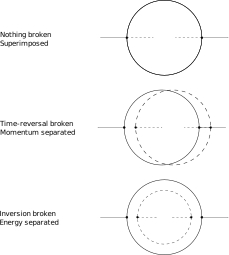
\includegraphics[width=0.75\textwidth]{figures/spinStructureWeyl}
  \caption{\label{fig:spinStructure} }
\end{figure}



\subsection{Symmetries}
In order to separate weyl cones in momentum, we introduce a pseuod spin degree of freedom, making the system 4x4.
We may then get solutions with the cones separated in momentum (or energy).
We may also ask what heppens if we try to separate tilted cones?

Firstly, in the most intuitive way to extend the 2x2 tilted cones to 4x4, we get that the cones tilt opposite direction, thus not superimposed even before separating in momentum.
They are after that simple to separate in momentum.
We might wonder if it makes sense to do it in this way.

The lattice model of the energy dispersion to explain tilted cones gives two cones separated in momentum, and tilting corresponds to ``bending'' the dispersion curves between them.
Maybe we therefore always have cones separated in momentum, and thus tilting superimposed does not make sense?
All depends on the origin of the tilt I believe.
Also, we must not confuse the global dispersion relation, to the Dirac cones which are expansions around the nodes.

Key to understand how spin behaves in all of this, and also maybe the symmetries.

To properly investigate the symmetry properties of the system, we must consider the 4x4, not 2x2 Hamiltonians.
While the 2x2 system does a goood job at describing a single cone, much important phsycis is lost when reducing the 4x4 Hamiltonian.
For example, the requirement that the total Berry curvature over the entire Briolluine zone is zero is not met for the 2x2 Hamiltonian, as it describes only one cone of a certain chirality.
The 4x4, however, includes two cones, which may in general be superimposed, thus conserving the total zero-divergence of the Berry curvature.
As a matter of fact, the inclusion of both cones is important also for symmetry considerations.

Let
\[
  H = v_{F} \tau _{x} \otimes \vec{\sigma} \vec{k},
\]
where \(\tau \) is some pseudo spin degree of freedom, transforming like \(\vec{r}\) under parity in time reversal.
This system describes two superimposed cones at the origin, with opposite chirality.
The effect of parity \(\mathcal{P}\) and time reversal \(\mathcal{T}\) is
\begin{table}[h]
  \centering
  \begin{tabular}{lcc}
    & \(\mathcal{P}\) & \(\mathcal{T}\)\\
    \hline
    \(\tau \) & - & +\\
    \(\sigma \) & + & -\\
    \(k\) & - & -
  \end{tabular}
\end{table}
\begin{equation}
  \label{eq:26}
  \begin{aligned}
    \mathcal{P} \tau \mathcal{P}^{\dagger} &= -\tau, & \mathcal{T} \tau \mathcal{T}^{\dagger} &= +\tau\\
    \mathcal{P} \sigma  \mathcal{P}^{\dagger} &= + \sigma,  & \mathcal{T} \sigma  \mathcal{T}^{\dagger} &= -\sigma \\
    \mathcal{P} k \mathcal{P}^{\dagger} &= -k, & \mathcal{T} k \mathcal{T}^{\dagger} &= -k
  \end{aligned}
\end{equation}
Obviously then, the Hamiltonian is both time reversal and parity invariant, as \(\mathcal{P} \mathcal{P}^{\dagger} = \mathcal{T} \mathcal{T}^{\dagger} = 1\).

A tilt term \(\tau _{x} \otimes \mathcal{I} \vec{\omega} _{0} \vec{k}\) breaks time reversal invariance, while maintaining parity invariance.
This is due to the two cones of opposite chirality tilting in opposite directions.

\begin{figure}[h]
  \centering
  \begin{tikzpicture}
    \draw[->] (-4, 0) -- (4, 0) node[right] {\(k\)};
    \draw[->] (0, 0) -- (0, 4) node[right] {\(E\)};

    % vf = 1, v0 = 0.8
    \draw[blue] (-3.5, 0.7) -- (0, 0) -- (2, 3.6) node[right] {\(\ket{\uparrow}\)} coordinate[pos=0.7] (a);
    \draw[red] (3.5, 0.7) node[right] {\(\ket{\downarrow }\)} -- (0, 0) -- (-2, 3.6)
    coordinate[pos=0.7] (b);

    \draw[->] (a) -- ++(1, 0);
    \draw[->] (b) -- ++(1, 0);
  \end{tikzpicture}
  \caption{Time reversal breaking in tilted system.
    Cross section in the tilt direction shown, with blue showing one cone and red the other.
    Black arrows indicate spin direction, which for \(\ket{\uparrow {}}\) is proporitional to  \(k\) while for \(\ket{\downarrow {}}\) is proportional to \( -k \).
  }
\end{figure}

The unperturbed Dirac Hamiltonian is Lorentz invariant, given that we consider an ``effective speed of light'', namely the Fermi velocity, instead of the actual speed of light \( c \).
Specifically, Lorentz invariance means invariance under the \emph{Lorentz group}.
The Lorentz group is the \( O(1,3) \) Lie group that conserves
\[
x_{\mu } x^{\mu } = t^2 - x^2 - y^2 - z^2,
\]
i.e. all isometries of Minkowski space.
More specifically, the group consists of all 3D rotations, \( O(3) \), and all \emph{boosts}.
A boost is a hyperbolic rotation from a spactial dimension to the temporal dimension.
If we now direct our focus at the Hamiltonian of the Dirac cone
\[
H = \pm v_{F} \vec{\sigma} \vec{p},
\]
we may easily show the Lorentz invariance of the system.
The time independent Schrodinger equation is
\begin{equation}
  \label{eq:44}
  H \ket{\psi } = E \ket{\psi } \implies (H^2 - E^2) \ket{\psi } = 0.
\end{equation}
As
\[
p^{\mu } = \left(\frac{E}{c}, \vec{p}\right),
\]
the operator in Eq. \eqref{eq:44} is nothing more than
\todo{ Make clear the matrix strucute here. There is an implicit identity matrix of size 2 }
\begin{equation}
  \label{eq:51}
  H^2-E^2 = v_{F}^2 \vec{p}^2 - c^2 \left(p^0\right)^2 ,
\end{equation}
where we used the anticommutation relation
\[
\{\sigma_{i}, \sigma_{j}\} =  2 \delta _{ij}
\]
of the Pauli matrices.
Using now the effective speed of light \( c=v_F \), Eq. \eqref{eq:51} is
\begin{equation}
  \label{eq:52}
  - v_F^2 p_{\mu } p^{\mu }.
\end{equation}

Consider now a \emph{tilted} Dirac cone
\begin{equation}
  \label{eq:53}
  H = \pm v_F \vec{\sigma} \vec{p} + \omega_{\perp} k_x,
\end{equation}
where we, without loss of generality, chose the tilt to be in the \( x \)-direction.




\begin{figure}[h]
  \centering
  \begin{tikzpicture}
    \begin{groupplot}[
      group style={group size=1 by 4},
      cycle list name=linestyles,
      ymin=-3, ymax=3,
      xmin=-3, xmax=3,
      ]
      % \foreach \paramwpp in {0,0.2,0.5,1} {
      % \foreach \paramalpha in {1, 0.8, 0.5, 0.2} {
      \pgfplotsinvokeforeach{1,2,3,4} {
        \nextgroupplot
        \newcommand{\paramwpp}{0}
        \newcommand{\paramalpha}{#1}
        % \newcommand{\paramalpha}{0.5}
        % \begin{axis}[
        %   cycle list name=linestyles,
        %   ymin=-3, ymax=3,
        %   ]
        \addplot {(\paramwpp - \paramalpha)  * x};
        % \foreach \n in {1,2,3,4} {
        %   \addplot {
        %     \paramwpp * x + sqrt(2 * \n * \paramalpha ^ 3 + x^2 * \paramalpha ^ 2)
        %   };
        %   \pgfplotsset{cycle list shift=-1}
        %   \addplot {
        %     \paramwpp * x - sqrt(2 * \n * \paramalpha ^ 3 + x^2 * \paramalpha ^ 2)
        %   };
        % }

        \pgfplotsinvokeforeach{1,2,3,4} {
          \addplot {
            \paramwpp * x + sqrt(2 * ##1 * \paramalpha ^ 3 + x^2 * \paramalpha ^ 2)
          };
          \pgfplotsset{cycle list shift=-1}
          \addplot {
            \paramwpp * x - sqrt(2 * ##1 * \paramalpha ^ 3 + x^2 * \paramalpha ^ 2)
          };
        }
        % \end{axis}
      }
    \end{groupplot}
  \end{tikzpicture}

  \caption{}
\end{figure}
